\documentclass[11pt,a4paper]{article}

\usepackage{amssymb}
\usepackage{amsmath}
\usepackage{lineno} 
\usepackage{dsfont}
\usepackage{amsfonts}
\usepackage{amsthm}
\usepackage{mathtools}
\usepackage{tikz}
\usetikzlibrary{shapes.geometric, arrows}
\usepackage{multirow}
\usepackage{physics}
\usepackage{graphicx}
\usepackage{caption}
\usepackage{subcaption}
\usepackage{listings}
\usepackage{relsize}
\usepackage{bigints}
\usepackage{natbib}
\usepackage[export]{adjustbox}
\usepackage[linesnumbered,commentsnumbered,ruled,vlined]{algorithm2e}
\usepackage[normalem]{ulem}
\usepackage{longtable}
\usepackage{float}
\usepackage{soul}
\usepackage{xcolor}

\graphicspath{{figures/}}

\setlength{\textheight}{24.0cm}
\setlength{\textwidth}{16.0cm}
\setlength{\parindent}{0.0cm}
\setlength{\topmargin}{-1.0cm}
\setlength{\oddsidemargin}{0.0cm}
\renewcommand{\baselinestretch}{1.}
\numberwithin{equation}{section}

% Title footnote command
\newcommand\funding[1]{\protect\\ \hspace*{15.37pt}{\bfseries Funding:} #1}
\newcommand\samethanks[1][\value{footnote}]{\footnotemark[#1]}

% Keywords command
\providecommand{\keywords}[1]
{
	\small	
	\textbf{\textit{Keywords---}} #1
}

\title{Modelling the influence of rhizodeposits on root water uptake}


\author{
	Andrew Mair\thanks{Department of Conservation of Natural Resources, NEIKER, Derio, Basque Country, Spain ({amair@neiker.eus, ORCID: 0000-0003-3847-5215})},\;  
	Lionel X Dupuy\thanks{Department of Conservation of Natural Resources, NEIKER \& IKERBASQUE, Derio, Basque Country, Spain ({ldupuy@neiker.eus, ORCID: 0000-0001-5221-9037})},\; 
	Mariya Ptashnyk\thanks{Department of Mathematics, School of Mathematical and Computer Sciences, Heriot-Watt University,  Scotland, United Kingdom ({m.ptashnyk@hw.ac.uk, ORCID: 0000-0003-4091-5080})},\;
	Emma Gomez Peral\thanks{Department of Conservation of Natural Resources, NEIKER, Derio, Basque Country, Spain ({egomez@neiker.eus})}  
	}
	

\date{} 

\begin{document}

\maketitle
\thispagestyle{empty}
\newpage	
\clearpage
\pagenumbering{arabic}
	
\begin{abstract} 
\end{abstract}

\keywords{}

\linenumbers

\section{Introduction}
For decades, advancing crop performance has been a key pursuit within agricultural research and, with the coupled pressures of an increasing global population and climate change, the need for improvements in yield and stress resilience are only increasing. Improving plant water use efficiency, whether from precipitation or irrigation, is a central focus and 3 facets of achieving this were previously outlined in~\citep{condon2004breeding}. The first two are to improve plant ability to convert transpired water into biomass, whilst also having crops partition more of this biomass into harvestable product. The final process, and the one focused on by this paper, is to enable the plant to take up a greater proportion of any water that is added to the soil. In this context the aim is to minimise losses of water from the regions of soil where uptake is possible, which may occur through evaporation or drainage to unvegetated depths~(Figure~\ref{figure: processes}). The part of the plant anatomy most relevant here is the root system, and an obvious morphological trait to consider when aiming to maximise plant access to water is the root system architecture (RSA). From the literature, the dominant ideotype proposed for stress-resistant rain-fed crops is a root system with sufficient lateral span at shallow depths to catch rainfall entering from above, but where the majority of resources are allocated to growing downward so that stores of water deep in the soil can be accessed during periods of drought~\citep{lynch2013steep, uga2013control, lynch2015opportunities}. Furthermore, the preference for deep roots persists to some extent in less water-limited environments because crop irrigation strategies involving access to deep soil water are less exposed to increasingly volatile rainfall patterns and facilitate the economic management of industrial scale cultivation~\citep{wasson2012traits}. Opinion is more nuanced when it comes to crops grown in environments where soil is shallow however. Here the priority is to capture water during infiltration before it runs off at bedrock and becomes unavailable, regardless of root length~\citep{tardieu2012any, wasson2012traits}.

Over a quarter of net fixed carbon among annual crops is apportioned to roots and, depending on species, between 25 to 70 percent of this is released into the soil in the form of rhizodeposits~\citep{mcgrail2020trait}. These rhizodeposits have been shown to materially affect the soil characteristics while also facilitating microbial colonisation, and the zone of soil falling under this influence is referred to as the rhizosphere. For example, rhizodeposit-induced changes to soil hydraulic properties have been frequently observed across a number of crop species. For Wheat, Maize and Barley the surface tension of soil water has been shown to decrease with increasing root exudate concentration~\citep{read1997surface, read2003plant, naveed2019surface} and in Maize and Wheat an increasing concentration of sorbed exudates in the soil was found to increase contact angle between water and the soil surface~\citep{ahmed2016drying, zickenrott2016efficient, benard2018pore, naveed2019surface}. Reductions in surface tension generally increase infiltration rates through the soil and increases in contact angle are known to impede soil-rewetting. The viscosity of soil water has also been found to be altered by increasing rhizodeposit concentration with increases reported for Maize and Barley~\citep{naveed2019surface}. From the mathematical description of saturated hydraulic conductivity, an increase in viscosity should translate as a decrease in saturated soil hydraulic conductivity, conversely however, for soils vegetated by Maize~\citep{feki2018influence}, Willow and Grass~\citep{leung2018plant} this has been observed as higher than that of fallow soil. Clearly, the combined effects of rhizodeposits on soil hydraulics are hard to untangle and their net effect on the availability of water to the root system, is difficult to ascertain and is likely to vary with environmental factors like rainfall pattern, evaporation rate and soil depth, and morphological or physiological traits like root system architecture and axial hydraulic conductivity. 

Improved knowledge of what rhizodeposit effects on soil hydraulics are beneficial or detrimental and under what conditions could prove useful to crop breeders in identifying target ideotypes for different agricultural zones where levels of available water and methods of irrigation differ. This paper aims to address this by taking a mathematical model for water transport and root water uptake in vegetated soil, which has been calibrated against for the effect of winter wheat exudates on soil hydraulic properties using results from an infiltration experiment, and investigating the effect of increased rhizodeposit concentration on uptake performance. The effect is considered for root systems of different ages in environments with varying levels of total rain and different patterns of rain delivery. 

\begin{figure}
	\centering
	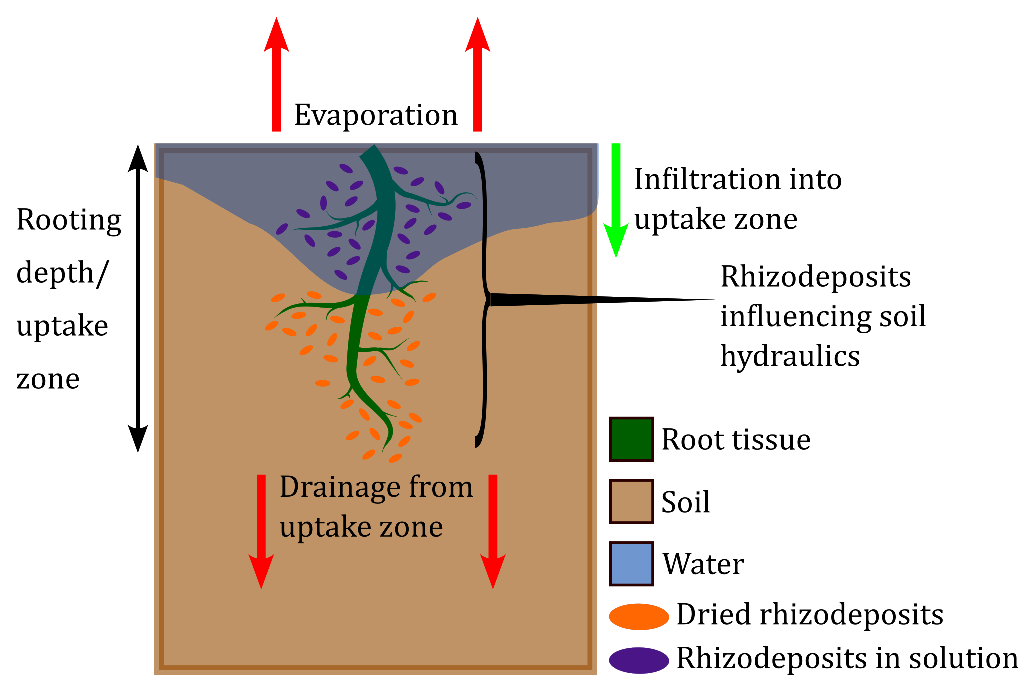
\includegraphics[width = 0.75\linewidth, keepaspectratio]{concept_figure_10_10_24.eps}
	\caption{Rhizodeposits and root water uptake. The uptake performance of a plant is affected by the availability of water within the rooted regions of the soil. This figure shows the various processes that determine levels of water availability, all of which are influenced by the presence of rhizodeposits.}
	\label{figure: processes}
\end{figure}

\section{Materials and Methods}
\subsection{A coupled model for soil water and rhizodeposit dynamics}\label{subsec: models}  
Assuming a soil domain~$\Omega = (-L, 0)$, with depth~$L$ and spatial variable~$x$, and temporal interval with final time~$T>0$, the relationship between soil hydraulics, root rhizodeposits, and root water uptake is modelled by coupling a modified Richards equation for water transport~\citep{richards1931capillary}:
\begin{linenomath*}
	\begin{equation}\label{model: water transport}
		\begin{aligned}
			\partial_t\theta(h; c_W, c_D) + \partial_x\mathbf{q}(h; c_W, c_D) &= - S(x,t) &x\in\Omega,~t\in(0, T],\\
			\mathbf{q}(h; c_W, c_D) &= g_0(h,t) &x = 0,~t\in(0, T],\\  
			-\mathbf{q}(h; c_W, c_D) &= g_L(h,t) &x = -L,~t\in(0, T],\\
			h &= h_0(x) & x\in\Omega,~t=0, 
		\end{aligned}
	\end{equation}
\end{linenomath*}	
with an advection diffusion equation for the dynamics of root rhizodeposits in solution
\begin{linenomath*}
	\begin{equation}\label{model: rhizodeposits in solution}
		\begin{aligned}
			\partial_t{\theta c_W} - \partial_x(\theta D_W\partial_xc_W - \mathbf{q}c_W) &= \rho\kappa_Wc_D - \theta\kappa_Dc_W + f(x, h)  
			&x\in\Omega,~t\in(0, T],\\
			 - (\theta D_W\partial_xc_W - \mathbf{q}c_W)&= 0 &x = 0,~t\in(0, T],\\
			 \theta D_W\partial_xc_W - \mathbf{q}c_W&= 0 &x = -L,~t\in(0, T],\\  
			 c_W & = c_{W,0}(x) &x\in\Omega,~t=0,	 
		\end{aligned}
	\end{equation}
\end{linenomath*}
and an ordinary differential equation for dried rhizodeposit concentration  
\begin{linenomath*}
	\begin{equation}\label{model: dried rhizodeposits}
		\begin{aligned}
			\rho\partial_tc_D &= \theta\kappa_Dc_W - \rho\kappa_Wc_D &x\in\Omega,~t\in(0, T],\\
			c_D & = c_{D,0} &x\in\Omega,~t=0.
		\end{aligned}
	\end{equation}
\end{linenomath*}
These component models~\eqref{model: water transport}, \eqref{model: rhizodeposits in solution} and \eqref{model: dried rhizodeposits} are solved for soil water pressure head~$h$~$[\text{L}]$, rhizodeposit concentration in solution~$c_W$~$[\text{ML}^{-3}]$ and rhizodeposit concentration dried to  the soil surface~$c_D$~$[\text{MM}^{-1}]$ respectively. In~\eqref{model: water transport}, soil water content is given by~$\theta$~$[\text{L}^3\text{L}^{-3}]$, root water uptake by~$S$~$[\text{T}^{-1}]$, and the flux conditions at the soil upper surface and base by~$g_0$ and $g_L$ respectively. The movement of water through the soil is driven by the Darcy-Buckingham flux~\citep{darcy1856fontaines}
\begin{linenomath*}
	\begin{equation}\label{model: water flux}
		\begin{aligned}
			\mathbf{q} = - K(h; c_W, c_D)\partial_x(h + x),
		\end{aligned}
	\end{equation}
\end{linenomath*}
with~$K$~$[\text{LT}^{-1}]$ being the hydraulic conductivity, and appears as the advective term in the flux of root rhizodeposits in solution. The remaining terms in~\eqref{model: rhizodeposits in solution} and~\eqref{model: dried rhizodeposits} are the rhizodeposit diffusion coefficient~$D_W$~$[\text{L}^2\text{T}^{-1}]$, the soil bulk density~$\rho$~$[\text{ML}^{-3}]$, a source term~$f$~$[\text{ML}^{-3}\text{T}^{-1}]$ for the release of rhizodeposits into the soil solution by the plant, and the rates at which dried rhizodeposits join the soil solution~$\kappa_W$~$[\text{T}^{-1}]$ and rhizodeposits in solution dry to the soil surface~$\kappa_D$~$[\text{T}^{-1}]$.
 
The influence of rhizodeposits is incorporated into the water transport and uptake model~\eqref{model: water transport} through modifications to the \cite{van1980closed} and \cite{mualem1976new} formulations of the functions for water content and hydraulic conductivity:
\begin{linenomath*}
	\begin{equation}\label{model: water retention}
		\begin{aligned}
			\theta(h; c_W, c_D) = \theta_r + (\theta_s-\theta_r)S_e(h; c_W, c_D),\\
		\end{aligned}
	\end{equation}
	\begin{equation}\label{model: hydraulic conductivity}
		\begin{aligned}
			K(h; c_W, c_D) = K^* + \alpha_KK_s(c_W, c_D)K_r(h; c_W, c_D).
		\end{aligned}	
	\end{equation}		
\end{linenomath*}
Here, the impact of rhizodeposits is built in through the effective soil saturation function~$S_e$ in~\eqref{model: water retention}, and the functions for saturated hydraulic conductivity~$K_s$~$[\text{LT}^{-1}]$ and relative hydraulic conductivity~$K_r$ in~\eqref{model: hydraulic conductivity}. The terms $\theta_r$ and~$\theta_s$ in~\eqref{model: water retention} give the residual and saturated soil water contents respectively and parameters~$K^*$~$[\text{LT}^{-1}]$ and~$\alpha_K$ are included in~\eqref{model: hydraulic conductivity} to account for the fact that 
water content and hydraulic conductivity values at a given pressure head are generally lower if a soil is wetting than if it is drying. This hysteresis exists because the processes that occur when a soil dries are generally governed by activity in the smaller pores whereas the wetting of a soil tends to be determined by the larger pores. Furthermore, the contact angles between the menisci and the soil surface are different depending on whether water is entering or draining from a pore~\citep{van2011hydraulic, zhou2013contact}. In~\eqref{model: water retention} the phenomenon of hysteresis is incorporated by the effective saturation
\begin{linenomath*}
	\begin{equation}\label{model: effective saturation}
		\begin{aligned}
			S_e(h;c_W, c_D)=\frac{1}{(1+|\alpha_{\theta}(c_W, c_D) h|^{n_{\theta}})^{m_{\theta}}}.
		\end{aligned}
	\end{equation}  
\end{linenomath*}
Here~$n_\theta$ and~$m_\theta=1-\frac{1}{n_\theta}$ are shape parameters and the parameter relating to inverse pore air entry pressure~$\alpha_{\theta}$~$[L^{-1}]$ takes different values depending on whether the soil is wetting or drying such that
\begin{linenomath*}
	\begin{equation}\label{model: inverse air entry pressure head}
		\begin{aligned}
			\alpha_{\theta}(c_W, c_D) =
			\begin{cases}
				\alpha_\theta^W(c_W, c_D) &\text{if wetting,}\\
				\alpha_\theta^D(c_W, c_D) &\text{if drying,}
			\end{cases}
		\end{aligned}
	\end{equation}
\end{linenomath*}
with~$\alpha_\theta^W \geq \alpha_\theta^D$~\citep{kool1987development}. Therefore, if at a given pressure head~$h_\Delta$ and  water content~$\theta_\Delta$ there is a switch from drying to wetting or vice versa, then the value of~$\alpha_{\theta}$ will also switch. To maintain the continuity of~$\theta$ when this happens, the residual and saturated water contents also switch between different values for wetting and drying:
\begin{linenomath*}
	\begin{equation}\label{model: hysteretic residual and saturated}
		\begin{aligned}
			\theta_{r}= 
			\begin{cases}
				\frac{(\theta_\Delta - \theta_{s,0}S_e(h_\Delta))}{1- S_e(h_\Delta)} &\text{if }\alpha_\theta=\alpha_\theta^W,\\
				\theta_{r,0} &\text{if }\alpha_\theta=\alpha_\theta^D, 
			\end{cases}\qquad
			\theta_{s} =
			\begin{cases}
				\theta_{s,0} &\text{if }\alpha_\theta=\alpha_\theta^W,\\
				\frac{\theta_\Delta - \theta_{r,0}(1-S_e(h_\Delta))}{S_e(h_\Delta)}&\text{if }\alpha_\theta =\alpha_\theta^D.
			\end{cases}			
		\end{aligned}
	\end{equation}
\end{linenomath*}   
This affects the value 
of~$K$ through the relative hydraulic conductivity
\begin{linenomath*}
	\begin{equation}\label{model: relative conductivity}
		\begin{aligned}
			K_r(h; c_W, c_D)
			=&
			\Bigg(\frac{2(\theta_{s, 0} - \theta_{r,0})S_e(h_\Delta; c_W, c_D) + \varepsilon\big(1-2S_e(h_\Delta; c_W, c_D)\big)}{2(\theta_{s,0} - \theta_{r,0})}\Bigg)^l\\
			&\cdot
			\Bigg(1 - \Bigg(1 - \Bigg(\frac{2(\theta_{s,0} - \theta_{r,0})S_e(h_\Delta; c_W, c_D) + \varepsilon\big(1-2S_e(h_\Delta; c_W, c_D)\big)}{2(\theta_{s,0} - \theta_{r,0})}\Bigg)^\frac{1}{m_\theta}\Bigg)^{m_\theta}\Bigg)^2,
		\end{aligned}
	\end{equation}
\end{linenomath*}
where the parameter~$l$ denotes the tortuosity of the porous structure. Moreover, hysteresis is also incorporated into~$K$ through a saturated hydraulic conductivity term that switches between values for wetting and drying soil~\citep{vogel1996hydrus}:
\begin{linenomath*}
	\begin{equation}\label{model: saturated hydraulic conductivity}
		\begin{aligned}
			K_{s}(c_W, c_D) =
			\begin{cases}
				K_s^W(c_W, c_D) &\text{if wetting,}\\
				K_s^D(c_W, c_D) &\text{if drying,}
			\end{cases}
		\end{aligned}
	\end{equation}
\end{linenomath*}
where~$K_s^D>K_s^W$. Like~\eqref{model: hysteretic residual and saturated}, the parameters~$K^*$ and~$\alpha_K$ in~\eqref{model: hydraulic conductivity} are also formulated so as to maintain the continuity of~$K$ if a switch between wetting and drying occurs at~$(h_\Delta,\theta_\Delta, K_\Delta)$~\citep{vogel1996hydrus}:
\begin{linenomath*}
	\begin{equation}\label{model: hydraulic conductivity hysteresis parameters}
		\begin{aligned}
			K^*&= 
			\begin{cases}
				K_s^WK_r(0)\Big(1-\frac{K_\Delta - K_s^WK_r(0)}{K_s^WK_r(h_\Delta) - K_s^WK_r(0)}\Big) \ &\text{if }K_s = K_s^W,\\
				 0 &\text{if }K_s = K_s^D,
			\end{cases}\\
			\alpha_K
			&=
			\begin{cases}
				\frac{K_\Delta-K_s^WK_r(0)}{K_s^WK_r(h_\Delta) - K_s^WK_r(0)}&\text{if }K_s = K_s^W,\\
				\frac{K_\Delta}{K_s^DK_r(h_\Delta)}&\text{if }K_s = K_s^D.
			\end{cases} 			
		\end{aligned}
	\end{equation}
\end{linenomath*}   

The surface tension of soil water~$\gamma$ and the contact angle~$\vartheta$ of its menisci with the pore surfaces have been shown by numerous studies to vary considerably with the concentration of rhizodeposits from a range of plant species~\citep{ahmed2016drying, naveed2018rhizosphere, naveed2019surface}. This study will focus on wheat plants and in this case there is evidence that rhizodeposits increase the soil-water contact angle~\citep{zickenrott2016efficient}, and decrease the surface tension of the soil solution~\citep{read2003plant}. To account for this within~$\theta$, the approach of~\cite{karagunduz2001influence} is employed and scaling factors are introduced into $\alpha_\theta$, such that for~$(c_W,c_D)\in[0,\infty)^2$, 
\begin{linenomath*}
	\begin{equation}\label{model: alpha vs rhizodeposits}
		\begin{aligned}
			\alpha_\theta^W(c_W,c_D) = \frac{\gamma(c_W)\cos(\vartheta_0)}{\gamma_0\cos(\vartheta(c_D))}\alpha_{\theta, 0}^W,
		\end{aligned}
		\quad
		\text{and}
		\quad
		\begin{aligned}
			\alpha_\theta^D(c_W) = 
			\frac{\gamma_0}{\gamma(c_W)}\alpha_{\theta, 0}^D,			 
		\end{aligned}
	\end{equation}
\end{linenomath*}
where~$\gamma_0$ and~$\vartheta_0$ are the surface tension and contact angle values in the absence of rhizodeposits, and~$\alpha_{\theta,0}^W$ and~$\alpha_{\theta,0}^D$ are the corresponding wetting and drying values of~$\alpha_\theta$. In the formulations of~\eqref{model: alpha vs rhizodeposits} a rhizodeposit-induced reduction in surface tension will decrease~$\alpha_\theta^W$ and increase~$\alpha_\theta^D$, which means the associated pressure head to a given water content will be decreased in wetting soil and increased in drying soil. Moreover, the assumption is made that soil-water contact angle will only have a material effect during the wetting of the soil, where an increase in contact angle will mean that the pressure head associated to a given water content during wetting is increased. In a similar way, to incorporate the effect of rhizodeposit-induced decreased surface tension and soil-water contact angle on~$K$, the saturated hydraulic conductivities are formulated so that, for~$(c_W,c_D)\in[0,\infty)^2$,
\begin{linenomath*}
	\begin{equation}\label{model: Ks vs rhizodeposits}
		\begin{aligned}
			K_s^Z = K_{s,0}^Z\Big(\frac{\gamma_0}{\gamma(c_W)}\Big)^\beta\frac{\cos(\vartheta(c_D))}{\cos(\vartheta_0)},
		\end{aligned}
	\end{equation}
\end{linenomath*}
where~$Z=W,D$. This formulation was informed by the experimental work in (Cite Emma's paper) where rhizodeposit induced reductions in surface tension increased hydraulic conductivity and this effect dominated over any rhizodeposit-induced increases in contact angle. The parameter~$\beta$ in~\eqref{model: Ks vs rhizodeposits} determines the extent to which such a rhizodeposit-induced reduction in surface tension will increase saturated hydraulic conductivity.

As in~\citep{vsimuunek2009modeling}, root water uptake in~\eqref{model: water transport} is modelled with a macroscopic sink term~$S$ incorporating water availability, root distribution, and potential plant transpiration~$\mathcal{T}_\text{p}$~$[LT^{-1}]$:
\begin{linenomath*}
	\begin{equation}\label{model: root water uptake}
		\begin{aligned}
			S(x, h) = \alpha_F(h)NRLD(x)\mathcal{T}_\text{p}\frac{1}{\max{(\omega(t),\omega_c)}}.
		\end{aligned}
	\end{equation}
\end{linenomath*}   
The dependence of uptake on the level of soil saturation is included in~$S$ through the dimensionless stress response function~$0\leq\alpha_f\leq1$, and  the plant's capacity to reach the water within the soil is accounted for by the normalised root length density~$NRLD$~$[L^{-3}]$, which is a continuous function that gives the distribution of root length within the soil. A measure of the global water stress experienced by the plant is given by the function
\begin{linenomath*}
	\begin{equation}\label{model: global water stress}
		\begin{aligned}
			\omega(t) = \int_\Omega\alpha_f(h(x, t))NRLD(x)dx
		\end{aligned}
	\end{equation}
\end{linenomath*}	
	
and the capacity of the plant to compensate for poor water availability in one soil region by increasing uptake in zones of higher saturation is reflected by~$\omega_c$~\citep{cai2018parameterization}. The boundary condition at the soil surface is
\begin{linenomath*}
	\begin{equation}\label{model: boundary condition soil surface}
		\begin{aligned}
			g_0(h, t) = K_e(h)\text{ET}_0 + RO(h,t) - P(t) 
		\end{aligned}
	\end{equation}
\end{linenomath*}
where~$K_e$~$[-]$ is a function that determines the proportion of total evapotranspiration that comes from evaporation,~$\text{ET}_0$~$[\text{LT}^{-1}]$ is the reference evapotranspiration,~$P$~$[\text{LT}^{-1}]$ the precipitation rate and~$RO$~$[\text{LT}^{-1}]$ is a function for the run-off of water that occurs when precipitation cannot enter the soil due to the surface already being fully saturated:
\begin{linenomath*}
	\begin{equation}\label{model: runoff function}
		\begin{aligned}
			RO(h,t) = P(t)\Big(1+\frac{\exp(a(\theta(h)-\theta_{s,0})) - 1}{\exp(a(\theta(h)-\theta_{s,0})) + 1}\Big). 
		\end{aligned}
	\end{equation}
\end{linenomath*}
Here the constant~$a>0$ is set to a large enough value so that if the surface is fully saturated ($\theta = \theta_{s, 0}$) then~$RO(t) = P(t)$. On the lower boundary~$x=-L$, the condition of free drainage is assumed, which translates as~$g_L(h) = K(h)$. The source term~$f$ in~\eqref{model: rhizodeposits in solution} for the release of rhizodeposits into the soil is formulated as follows:
\begin{linenomath*}
	\begin{equation}\label{model: rhizodeposit release}
		\begin{aligned}
			f(x,h) = \lambda\theta(h) SAD(x),
		\end{aligned}	
	\end{equation}
\end{linenomath*}
where~$\lambda$~$[\text{M}\text{L}^{-2}\text{T}^{-1}]$ is the rate at which rhizodeposits are released from the surface of the root and $SAD$~$[\text{L}^{-1}]$ is the root surface area density, a continuous function representing the distribution of root surface area throughout the soil. Expressions for any functions that have not been explicitly discolsed in this paper can be found in the supplementary material.

\subsection{Parametrisation and Calibration}\label{subsec: parametrisation and calibration}  	      
To explicitly model the ways in which rhizodeposits induce a reduction in soil water surface tension~$\gamma$, and an increase in the contact angle~$\vartheta$ between menisci and the soil pore surface, the data of~\cite{read2003plant} and~\cite{zickenrott2016efficient} was used to fit the following functions:
\begin{linenomath*}
	\begin{equation}\label{model: surface tension}
		\begin{aligned}
			\gamma(c_W) = 47.5 +\frac{72.86-47.5}{1 + \exp(18.79(c_W-0.36))},
		\end{aligned}
	\end{equation}
	and
	\begin{equation}\label{model: contact angle}
		\begin{aligned}
			\vartheta(c_D) = \frac{3.529}{18}\pi(1+\exp(-1879.14c_D))^{-4.39}.
		\end{aligned}
	\end{equation}
\end{linenomath*}
These functions return~$\gamma_0=\gamma(0)=72.86\text{mNm}^{-1}$ and~$\vartheta_0 = \vartheta(0) = 0.0294\text{rad}$ as the surface tension and contact angle when there are no rhizodeposits present. The soil type and crop species considered in all model simulations were sandy loam and winter wheat, and the majority of the values that were required to parametrise the models accordingly were taken from existing literature, see supplementary material for the specific values and from where they were sourced. 

The remaining parameter values to source were then the rates at which dried rhizodeposits join the soil water solution~$\kappa_W$ and rhizodeposits in solution dry to the pore surface~$\kappa_D$, and also the parameter~$\beta$ that controls the size of the increase in saturated hydraulic conductivity that is brought about by a rhizodeposit-induced reduction in surface tension. However, the values of these 3 parameters were recently approximated in the work of EMMA ET AL. In that study, an experimental setup was used in which 4 chambers were filled with 3 distinctly treated layers of Nafion a transparent artificial soil. The top layer was saturated with water and dye, the layer at the bottom was saturated with only water and the particles of the central layer were completely dry. In one of the chambers winter wheat rhizodeposits were then added to the water and dye solution of the upper layer. In the second chamber dried exudates were added only to the dry middle layer of the chamber. The third chamber had rhizodeposits in the solution in the upper layer as well as dried rhizodeposits in the central layer, and the fourth chamber was left as the control with no rhizodeposits added. Infiltration was left to occur for 5 days within these 4 chambers and, to assess the effect of rhizodeposits, the dye concentration in the lower layer of each chamber was recorded at regular intervals. To approximate~$\kappa_D$,~$\kappa_W$ and~$\beta$,~EMMA ET AL used the model system~\eqref{model: water transport}-\eqref{model: dried rhizodeposits}, along with an advection diffusion equation for dye concentration within the chamber, to simulate their experimental procedure. Bayesian optimisation~\cite{brochu2010tutorial} was then employed to run simulations of these models and search the parameter space of~$(\kappa_D,\kappa_W, \beta)$ to approximate the values that allowed the model system to best reproduce the results of the experiment. Further details of this experimental setup and the calibration procedure involving Bayesian optimisation can be found in~(EMMA ET AL) and the supplementary material.

The functions for normalised root length density~$NRLD$ and surface area density~$SAD$ were constructed for 3 winter wheat root systems of ages 6, 15 and 30 days (ADD FIGURE?). Architectures of these root systems were generated from CRootBox~\citep{schnepf2018crootbox} and the methods previously employed and described in~\citep{mair2022model, mair2023can, mair2023mathematical} were used to convert this architecture data into density functions for the distributions of root length and surface area within the 3-dimensional spatial domain that enclosed all 3 root systems. These functions were then averaged laterally across the 3D domain to produce~$NRLD$ and~$SAD$ as functions of 1D space~$(-L,0)$ where~$L = 52.973\text{cm}$ is the greatest depth reached by any root of the 3 systems. The exact parameter settings that were used within CRootBox to simulate the different root systems are shown in the supplementary material. 

\subsection{Simulated scenarios}
To investigate the impact of rhizodeposits on root water uptake performance, the model system~\eqref{model: water transport},~\eqref{model: rhizodeposits in solution} and~\eqref{model: dried rhizodeposits} was separately parametrised for each age of root system. For every root system parametrisation, 6 precipitation regimes were considered. In 3 of these regimes the precipitation function~$P$ was formulated to deliver a total of~$0.12\text{cm}$ rainfall over a time period of~$T=3\text{d}$ days, delivered in either 1, 2 or 3 rainfall events. In order to ensure total precipitation remained the same across all patterns, each time the total number of rainfall events was increased by 1 the duration of each rainfall event decreased by~$25\%$, along with a corresponding decrease in the rainfall rate. The other 3 precipitation regimes were defined in the same way, but with total rainfall set to~$0.28\text{cm}$. Figures~\ref{figure: almeria_precip_evap_up} and~\ref{figure: Madrid_precip_evap_up}~(a)-(c) provide a visual representation of the precipitation function~$P$ for the 6 different rainfall patterns. In each scenario, initial water content was set to a uniform value of~$\theta(h_0) = 0.69$ throughout the domain. In the non-control scenarios that included rhizodeposits, the initial concentration of rhizodeposit in solution was set so that in the depths of soil occupied by roots~$C_{W,0}=2.5\text{mgcm}^{-3}$ but in the depths without roots~$C_{W,0}=0\text{mgcm}^{-3}$. Assuming an initial equilibrium between the dynamics of dried rhizodeposits and rhizodeposits in solution, initial dried rhizodeposit concentration was set so that~$C_{D,0}=5.2\times10^{-4}\text{mgcm}^{-3}$ in domain depths with roots, and~$C_{D,0}=0\text{mgcm}^{-3}$ in depths without vegetation. Explicit mathematical formulations for all of these initial conditions and of~$P$ for each precipitation regime is given in the supplementary material. Infiltration simulations were then obtained for each root system and precipitation pattern combination, both with and without the incorporation of rhizodeposit influence, and data on soil water distribution and root water uptake were gathered.    

\subsection{Computations}
Numerical solutions for pressure head, rhizodeposits in solution and dried rhizodeposits were obtained from the model system~\eqref{model: water transport},~\eqref{model: rhizodeposits in solution},~\eqref{model: dried rhizodeposits} using a conformal finite element method and an implicit Euler discretisation in time. The cells of the 1D domain discretisation were each~$0.59273\text{cm}$ in length, and the time step size was~$ 0.001\text{d}$. Linearisation of the functions for water content and hydraulic conductivity in~\eqref{model: water transport} was carried out using the L-scheme of~\cite{list2016study}. The numerical method was implemented using the FEniCS library~\cite{AlnaesBlechta2015a} and the algorithms to construct NRLD and SAD from CRootBox architectures were run in Python 3 using the libraries NumPy and SciPy~\citep{harris2020array}. The visualisations of 1D root density profiles, water distributions and flux strength were generated from Paraview~\citep{ahrens2005paraview}.

\section{Results}

\subsection{General rhizodeposit effects on soil water dynamics and uptake}
For all rainfall patterns in the regimes of both lower and higher total precipitation, and all root system ages, following the onset of a rainfall event, the presence of rhizodeposits within soil was found to induce a boost in uptake to a rate higher than that exhibited in the situation without rhizodeposits~(Figures~\ref{figure: almeria_precip_evap_up}~and~\ref{figure: Madrid_precip_evap_up}~(g)-(i)). 
Moreover, for all root systems in all precipitation conditions the presence of rhizodeposits in the soil was shown to reduce evaporation from the upper soil surface to a lower rate, and this effect was maintained for the remainder of the entire simulation time~(Figures~\ref{figure: almeria_precip_evap_up}~and~\ref{figure: Madrid_precip_evap_up}~(g)-(i)).
Despite this, however, it was not true in all scenarios that uptake in the presence of rhizodeposits was maintained at a higher rate than without rhizodeposits for the entire simulation.

Figures~\ref{figure: almeria_3_events_fluxes}~and~\ref{figure: madrid_1_event_fluxes} show that the presence of rhizodeposits increased the strength of the downward water flux in the scenarios of a lower total precipitation delivered over 3 rainfall events and a higher total precipitation delivered in one event. It can also be seen that this increased flux led to an accelerated arrival of water to the rooted zone compared to the non-rhizodeposit case, and a greater proportion of water reaching deeper regions of the soil at earlier times. This was true for all total rainfall quantities and delivery patterns but Figures~\ref{figure: almeria_3_events_fluxes} and~\ref{figure: madrid_1_event_fluxes} show the regimes under which this effect was most weakly and strongly observed respectively.

Considering root systems of all ages, there was a general trend that the percentage positive change in total water uptake, which came from including rhizodeposits in the model, decreased as the amount of total rainfall in the 3 day simulation was increased~(Figure~\ref{figure: uptake_age_intensity}). In addition, when fixing total rainfall and considering the pattern by which it was delivered, it is also true that the positive effect of rhizodeposits on total water uptake was reduced as the quantity of precipitation delivered per event increased.

The remaining subsections of this results section provide more precise detail on how the strength and consequences of these rhizodeposit effects were felt differently for root systems of different ages.

\subsection{Rhizodeposits and the uptake performance of plants with shallower root systems}
In all 3 rainfall patterns of the regime with lower total rainfall~(0.12cm), the uptake rates of the 6 and 15-day old wheat plants, which have shallower root architectures~(Figure~\ref{figure: almeria_3_events_fluxes}/MATLAB Figure), are higher when rhizodeposits are present than when they are not, and this is true at all time points~(Figure~\ref{figure: almeria_precip_evap_up}). However, in the precipitation pattern where all 0.12cm is delivered in a single event, it can also be seen from Figure~\ref{figure: almeria_precip_evap_up} that this difference in uptake rate had almost closed by the end of the 3 day period. Nevertheless, in all these conditions, with total rainfall at 0.12cm, total water uptake over the 3 day period is obviously still higher for the root systems where rhizodeposits are present than those where they are not~(Table~\ref{table: lower rainfall total uptake}).

In the regime where a higher total precipitation is delivered, if the 0.28cm is split between 2 or 3 rainfall events, then the 6 and 15-day old root systems with rhizodeposits also had higher total root water uptake than without rhizodeposits~(Table~\ref{table: lower rainfall total uptake}). But, although under all 3 different precipitation patterns of the 0.28cm the uptake of these shallower root systems with rhizodeposits initially assumes a rate that is higher than that for when rhizodeposits are not present, eventually the uptake rates of the systems without rhizodeposits overtake and maintain a higher value until the end of the simulation~(Figure~\ref{figure: Madrid_precip_evap_up}). The timing of this overtake is earliest for the precipitation pattern in which all 0.28cm are delivered in one event, and, in this case, the difference in the uptake rates becomes so large that the 6 and 15-day old root systems actually return larger total water uptakes without rhizodeposits than with them~(Table~\ref{table: higher rainfall total uptake}). This effect can also be seen in Figure~\ref{figure: uptake_age_intensity} which shows that the percentage change in total water uptake that is induced by the presence of rhizodeposits is negative in the case where root systems are shallow and 0.28cm of precipitation is delivered in one event.  
 

\subsection{Rhizodeposits and the uptake performance of plants with deeper root systems}
For the 30-day old root system, which had the deepest rooting depth, the uptake rate when rhizodeposits were present was higher, at all points in time, than when rhizodeposits were not considered, and this was true for the regimes with both lower and higher total rainfall and across all precipitation patterns. As a result, total root water uptake for these deeper root systems over the 3 day period was greater when rhizodeposits were present than when they were not~(Figures~\ref{figure: almeria_precip_evap_up}~and~\ref{figure: Madrid_precip_evap_up}). 

A seemingly more anomalous result, however, was that within certain time intervals of the 3 day simulations (if not the entire simulation), for systems with and without rhizodeposits, the uptake rate of the 15-day old root system was higher than that of the 30-day old~(Figures~\ref{figure: almeria_precip_evap_up}~and~\ref{figure: Madrid_precip_evap_up}). In fact, when rhizodeposits were not present, for every case where total rainfall was 0.28cm or where all 0.12cm of total rainfall was delivered in one event, the greatest total uptake over the 3 days was by the 15-day old root system~(Table~\ref{table: lower rainfall total uptake}~column~2~and,~Table~\ref{table: higher rainfall total uptake}~columns~2,~4,~6). Furthermore, the rhizodeposit-enhanced water flux in the soil vegetated by the 15-day old root system was stronger than in the soil vegetated by the 30-day old plant~(Figure~\ref{figure: madrid_1_event_fluxes}).


  
\begin{figure}
	\centering
	\begin{subfigure}{0.32\textwidth}
		\includegraphics[width = \linewidth, keepaspectratio] {pr_ppat1ptot0_12.eps}
		\caption{}
	\end{subfigure}
	\begin{subfigure}{0.32\textwidth}
		\includegraphics[width = \linewidth, keepaspectratio] {pr_ppat2ptot0_12.eps}
		\caption{}
	\end{subfigure}
	\begin{subfigure}{0.32\textwidth}
		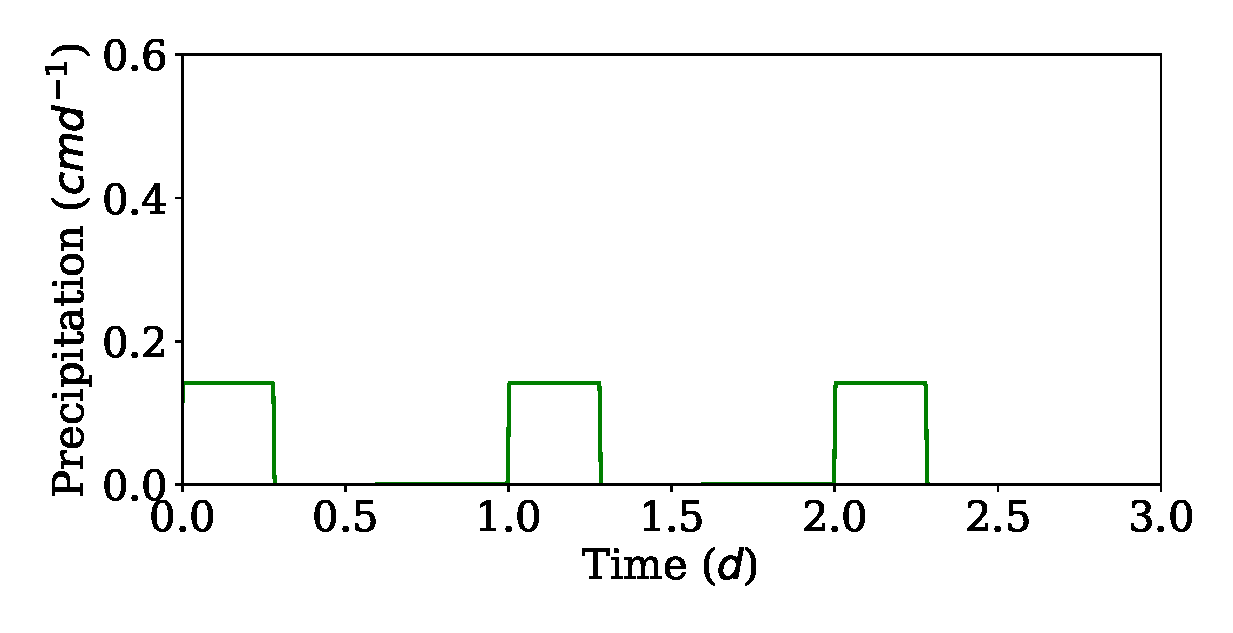
\includegraphics[width = \linewidth, keepaspectratio] {pr_ppat3ptot0_12.eps}
		\caption{}
	\end{subfigure}\\
	\begin{subfigure}{0.32\textwidth}
		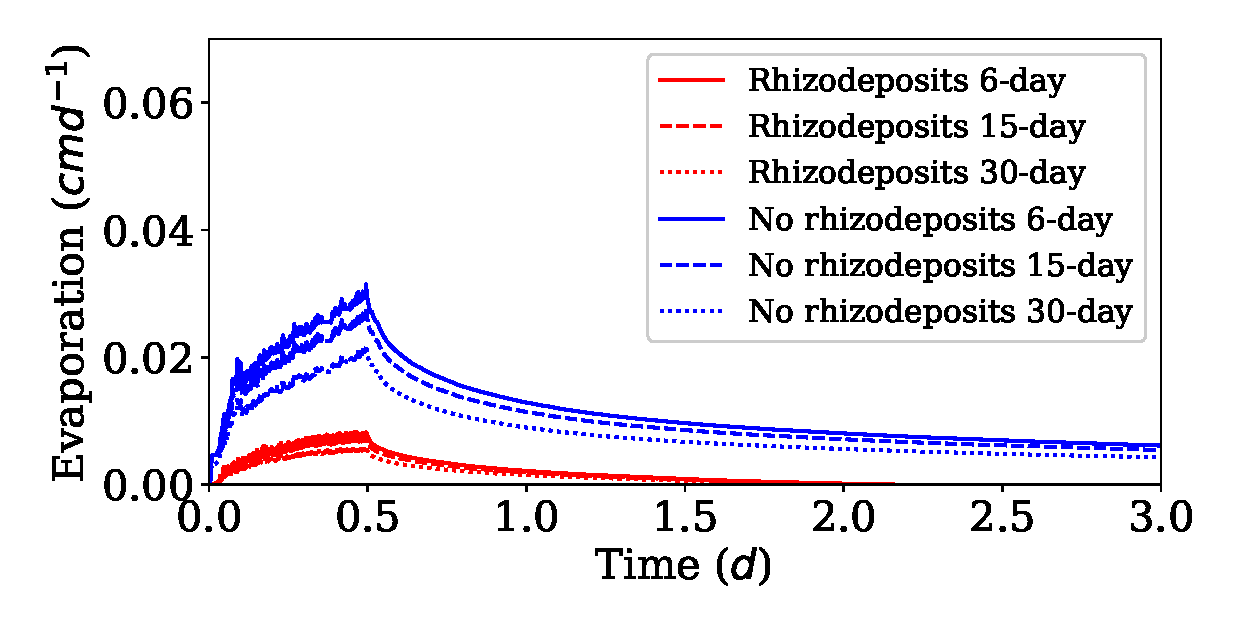
\includegraphics[width = \linewidth, keepaspectratio] {ev_ppat1ptot0_12.eps}
		\caption{}
	\end{subfigure}
	\begin{subfigure}{0.32\textwidth}
		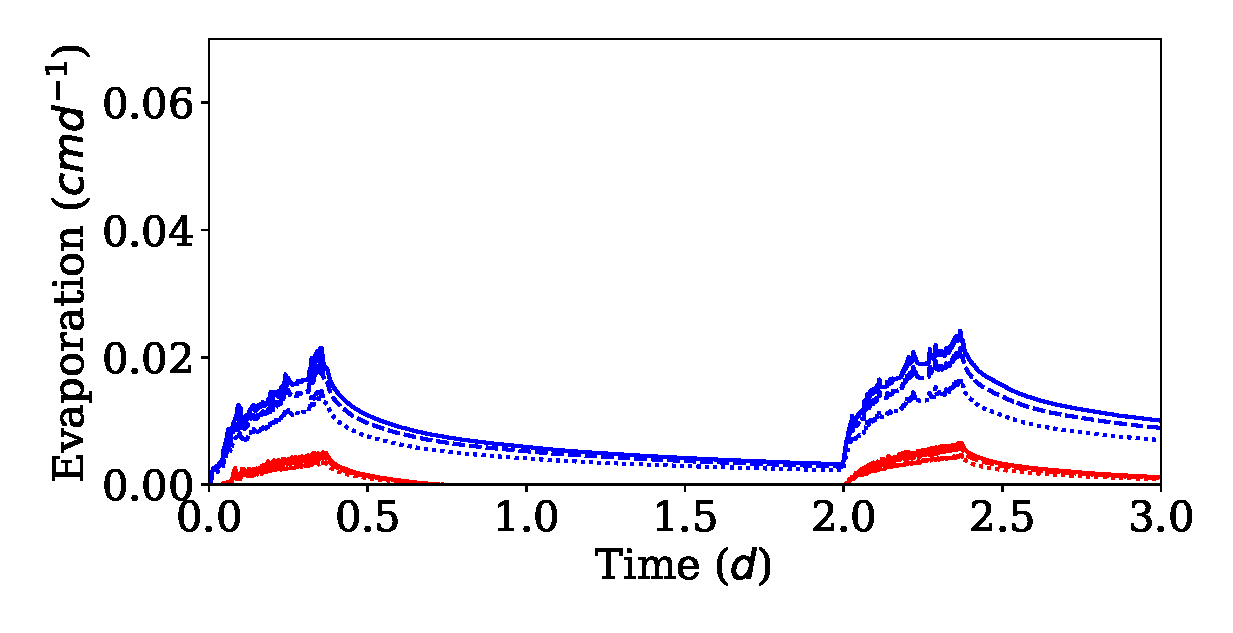
\includegraphics[width = \linewidth, keepaspectratio] {ev_ppat2ptot0_12.eps}
		\caption{}
	\end{subfigure}
	\begin{subfigure}{0.32\textwidth}
		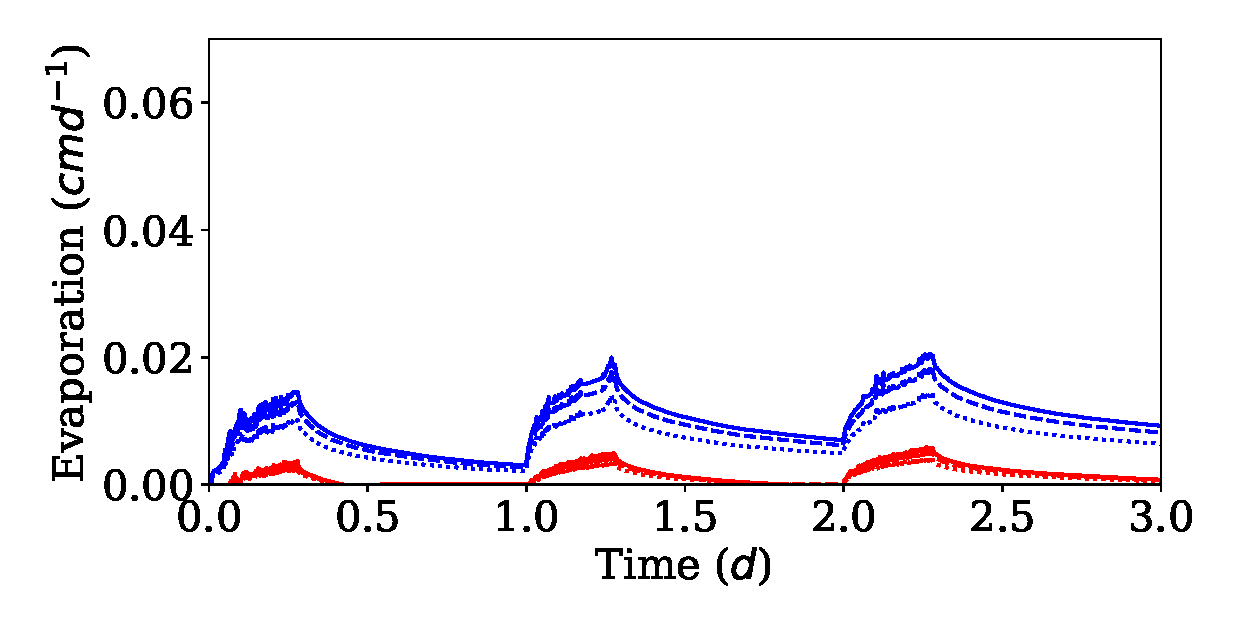
\includegraphics[width = \linewidth, keepaspectratio] {ev_ppat3ptot0_12.eps}
		\caption{}
	\end{subfigure}\\
	\begin{subfigure}{0.32\textwidth}
		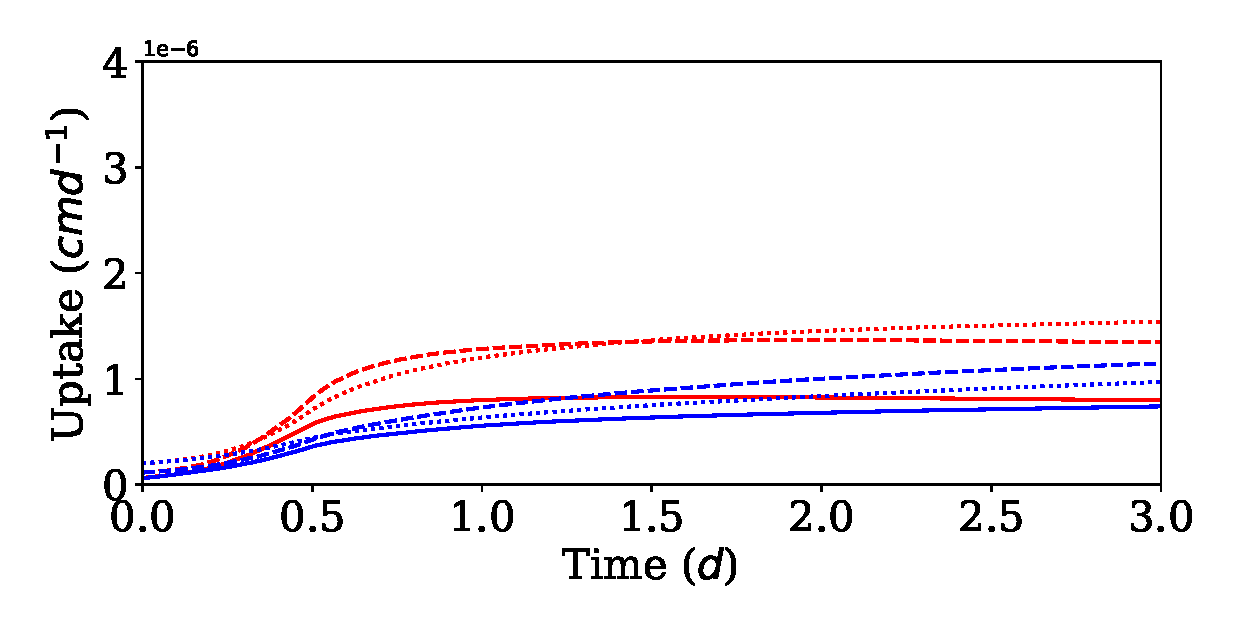
\includegraphics[width = \linewidth, keepaspectratio] {up_ppat1ptot0_12.eps}
		\caption{}
	\end{subfigure}
	\begin{subfigure}{0.32\textwidth}
		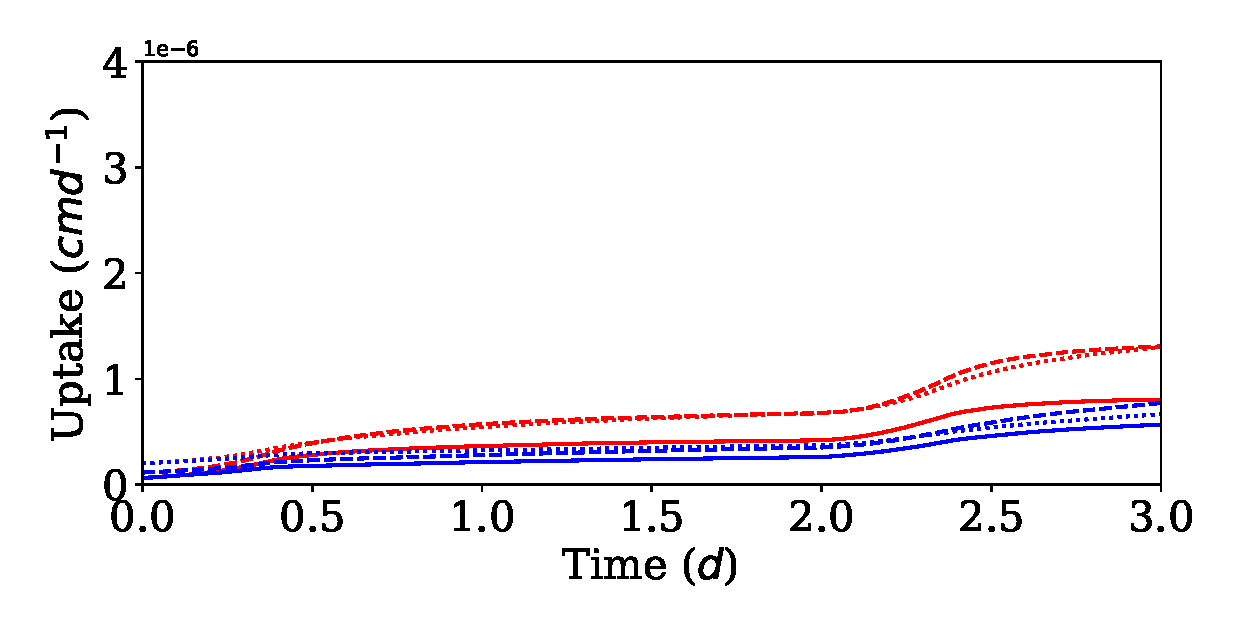
\includegraphics[width = \linewidth, keepaspectratio] {up_ppat2ptot0_12.eps}
		\caption{}
	\end{subfigure}
	\begin{subfigure}{0.32\textwidth}
		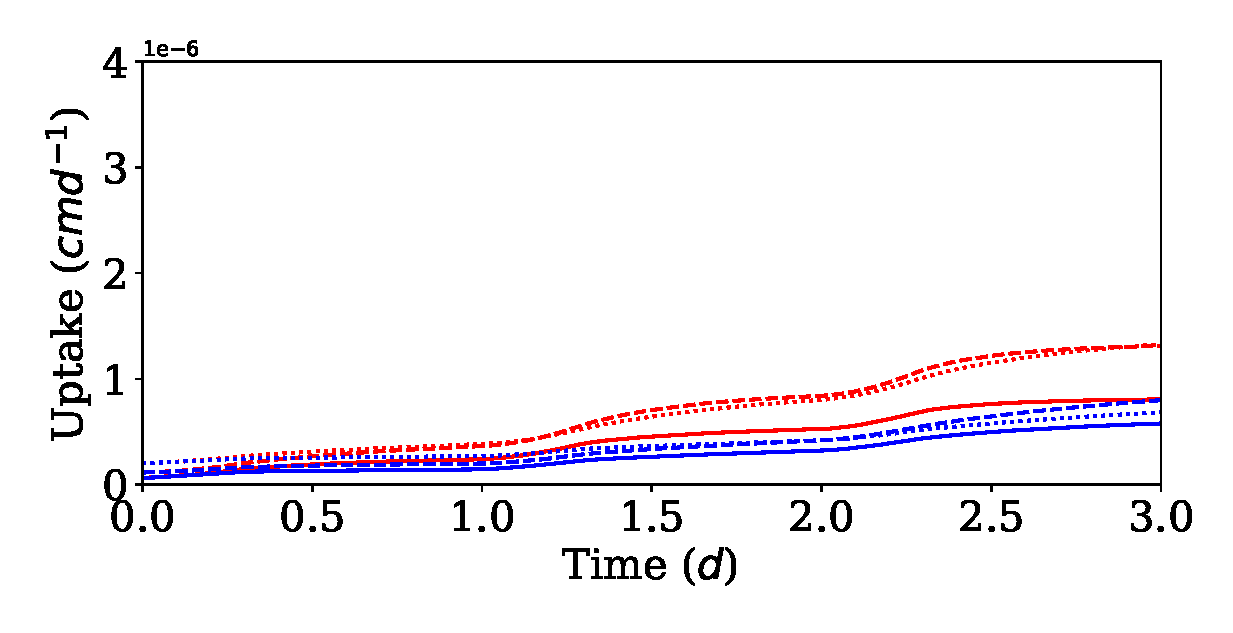
\includegraphics[width = \linewidth, keepaspectratio] {up_ppat3ptot0_12.eps}
		\caption{}
	\end{subfigure}
	\caption{The influence of rhizodeposits on root water uptake under different precipitation regimes of a lower-rainfall environment. Plots (a)-(c) show the precipitation patterns considered. The plots (d)-(f) lying directly below show the evaporation rates corresponding to each pattern and for soils occupied by each age of root system with or without rhizodeposits present. Similarly plots (g)-(i) show the corresponding uptake rates of each root system, with and without rhizodeposits present}
	\label{figure: almeria_precip_evap_up}
\end{figure}

\begin{figure}
	\centering
	\begin{subfigure}{0.32\textwidth}
		\includegraphics[width = \linewidth, keepaspectratio] {pr_ppat1ptot0_28.eps}
		\caption{}
	\end{subfigure}
	\begin{subfigure}{0.32\textwidth}
		\includegraphics[width = \linewidth, keepaspectratio] {pr_ppat2ptot0_28.eps}
		\caption{}
	\end{subfigure}
	\begin{subfigure}{0.32\textwidth}
		\includegraphics[width = \linewidth, keepaspectratio] {pr_ppat3ptot0_28.eps}
		\caption{}
	\end{subfigure}\\
	\begin{subfigure}{0.32\textwidth}
		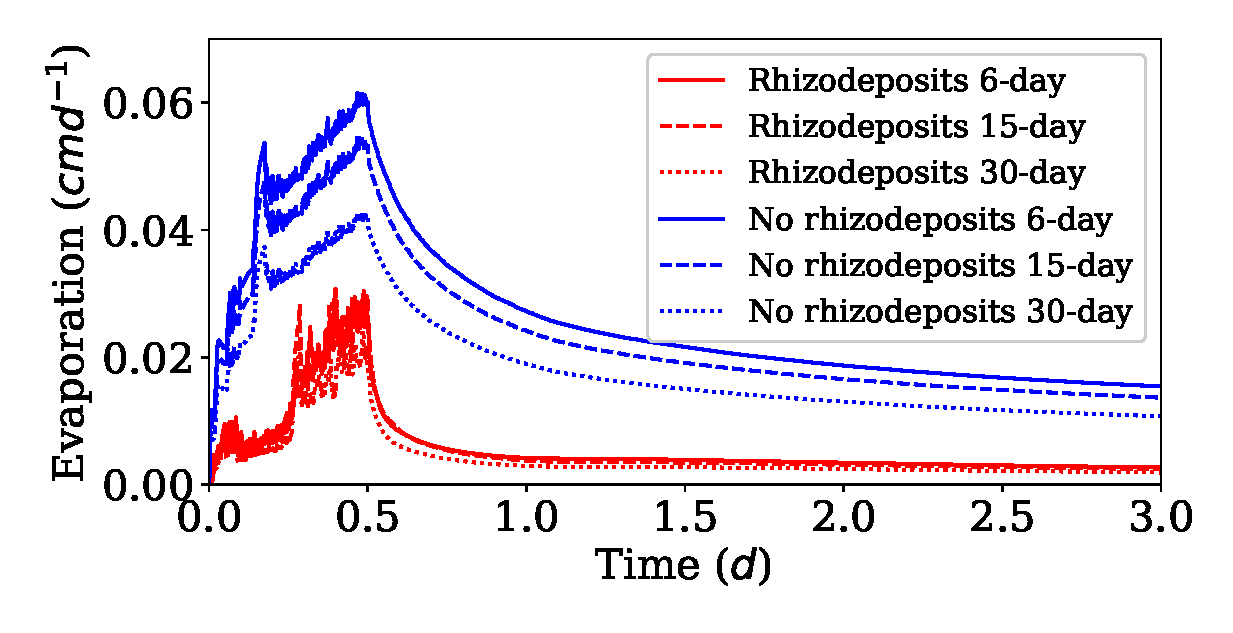
\includegraphics[width = \linewidth, keepaspectratio] {ev_ppat1ptot0_28.eps}
		\caption{}
	\end{subfigure}
	\begin{subfigure}{0.32\textwidth}
		\includegraphics[width = \linewidth, keepaspectratio] {ev_ppat2ptot0_28.eps}
		\caption{}
	\end{subfigure}
	\begin{subfigure}{0.32\textwidth}
		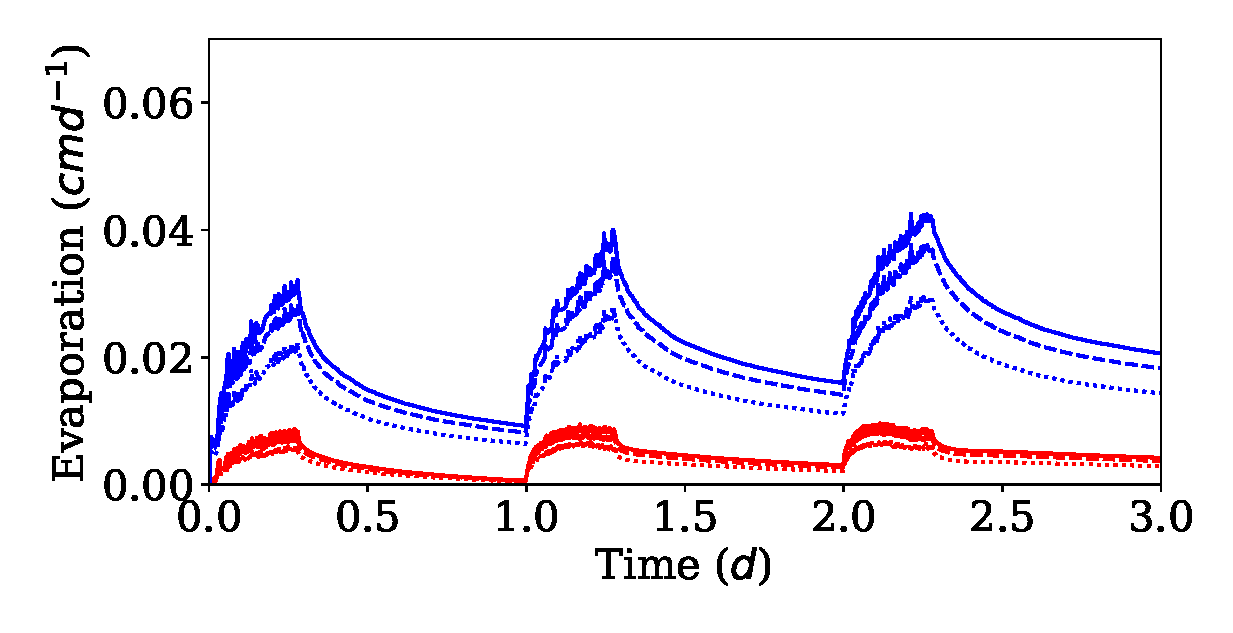
\includegraphics[width = \linewidth, keepaspectratio] {ev_ppat3ptot0_28.eps}
		\caption{}
	\end{subfigure}\\
	\begin{subfigure}{0.32\textwidth}
		\includegraphics[width = \linewidth, keepaspectratio] {up_ppat1ptot0_28.eps}
		\caption{}
	\end{subfigure}
	\begin{subfigure}{0.32\textwidth}
		\includegraphics[width = \linewidth, keepaspectratio] {up_ppat2ptot0_28.eps}
		\caption{}
	\end{subfigure}
	\begin{subfigure}{0.32\textwidth}
		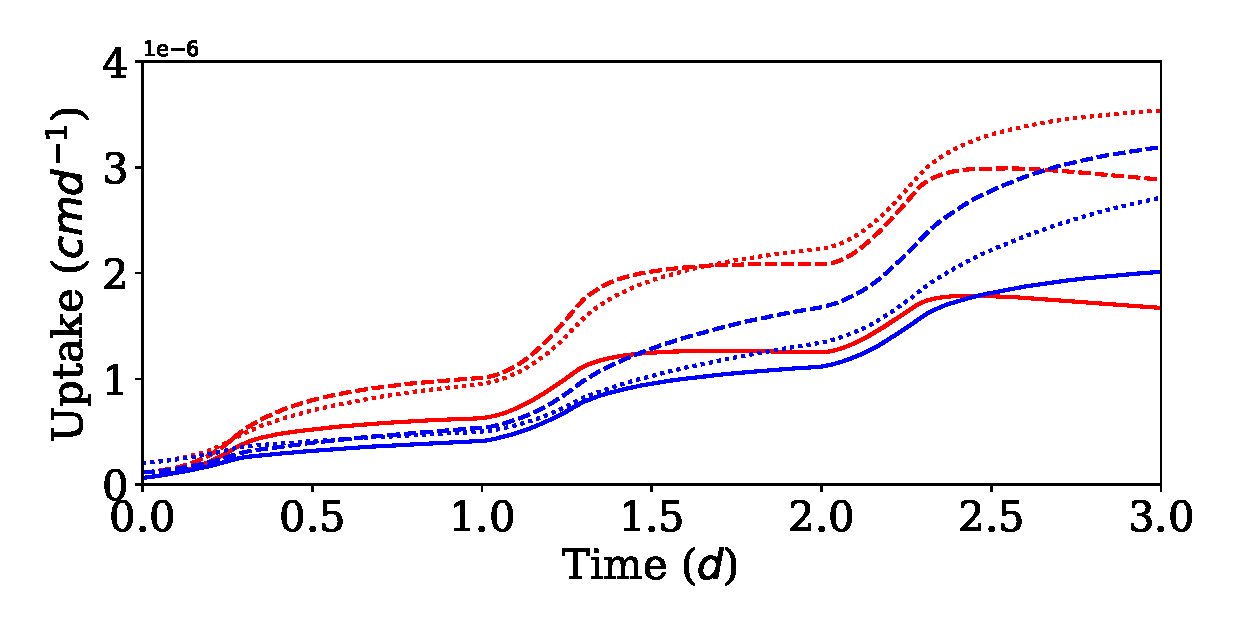
\includegraphics[width = \linewidth, keepaspectratio] {up_ppat3ptot0_28.eps}
		\caption{}
	\end{subfigure}
	\caption{The influence of rhizodeposits on the evolution of soil water content and flux over time under the single-event pattern of the higher total rainfall regime. The figures of the leftmost column shows the normalised root length density profiles of each plant with age increasing downwards. The remaining columns show snapshots of the water content dynamics (with and without rhizodeposits) at different time points of the simulation where each row relates to soil vegetated by the roots of each age of plant. The arrows illustrate the strength of the flow at each time point of the various conditions}
	\label{figure: Madrid_precip_evap_up}
\end{figure}

\begin{table}
	\centering
	\smaller
	\begin{tabular}{{ |p{3cm}||p{1.55cm}|p{1.55cm}|p{1.55cm}|p{1.55cm}|p{1.55cm}|p{1.55cm}||}}
		\hline
		\multicolumn{1}{|l||}{Total rainfall} &
		\multicolumn{6}{|c||}{0.12cm}\\
		\hline
		\multicolumn{1}{|l||}{Rainfall distribution} &
		\multicolumn{2}{|c|}{1 event} &
		\multicolumn{2}{|c|}{2 events} &
		\multicolumn{2}{|c||}{3 events}\\
		\hline
		Rhizodeposits & No & Yes & No & Yes & No & Yes\\
		\hline
		Total uptake: 6-day old plant (cm)& $1.67\times10^{-6}$ & $2.12\times10^{-6}$ & $8.35\times10^{-7}$ & $1.31\times10^{-6}$ & $8.49\times10^{-7}$ & $1.32\times10^{-6}$\\
		\hline
		Total uptake: 15-day old plant (cm)& $2.38\times10^{-6}$ & $3.44\times10^{-6}$ & $1.10\times10^{-6}$ & $2.05\times10^{-6}$ & $1.12\times10^{-6}$ & $2.06\times10^{-6}$\\
		\hline
		Total uptake: 30-day old plant (cm)& $2.08\times10^{-6}$ & $3.55\times10^{-6}$ & $1.16\times10^{-6}$ & $2.02\times10^{-6}$ & $1.17\times10^{-6}$ & $2.03\times10^{-6}$\\
		\hline
	\end{tabular}
	\caption{Total uptake of each root system with and without rhizodeposits for each rainfall distribution of the lower-rainfall regime.}
	\label{table: lower rainfall total uptake}
\end{table}



\begin{figure}
	\centering
	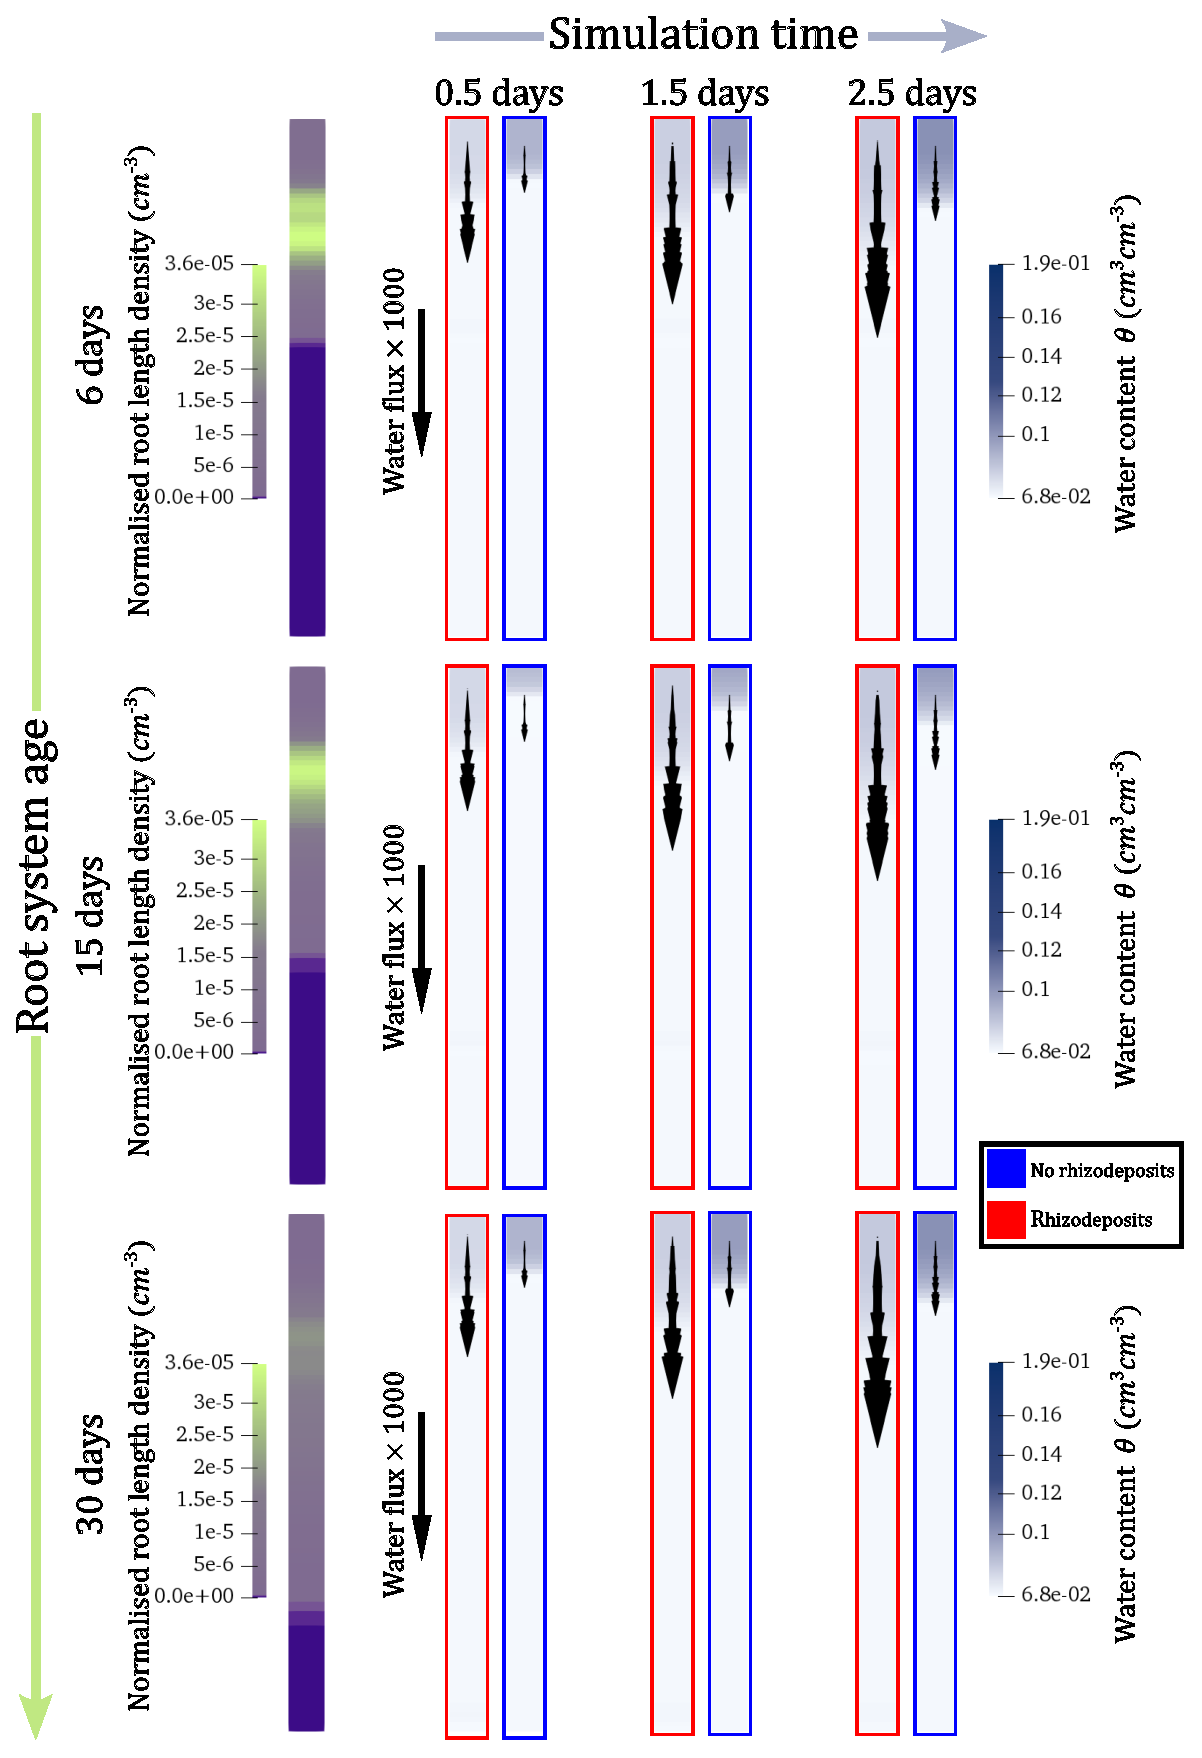
\includegraphics[width = 0.75\linewidth, keepaspectratio]{almeria_3_events.eps}
	\caption{The influence of rhizodeposits on the evolution of soil water content and flux over time under the 3-event pattern of the lower total rainfall regime. The figures of the leftmost column shows the normalised root length density profiles of each plant with age increasing downwards. The remaining columns show snapshots of the water content dynamics (with and without rhizodeposits) at different time points of the simulation where each row relates to soil vegetated by the roots of each age of plant. The arrows illustrate the strength of the flow at each time point of the various conditions}
	\label{figure: almeria_3_events_fluxes}
\end{figure}



\begin{table}
	\centering
	\smaller
	\begin{tabular}{{ |p{3cm}||p{1.55cm}|p{1.55cm}|p{1.55cm}|p{1.55cm}|p{1.55cm}|p{1.55cm}||}}
		\hline
		\multicolumn{1}{|l||}{Total rainfall} &
		\multicolumn{6}{|c||}{0.28cm}\\
		\hline
		\multicolumn{1}{|l||}{Rainfall distribution} &
		\multicolumn{2}{|c|}{1 event} &
		\multicolumn{2}{|c|}{2 events} &
		\multicolumn{2}{|c||}{3 events}\\
		\hline
		Rhizodeposits & No & Yes & No & Yes & No & Yes\\
		\hline
		Total uptake: 6-day old plant (cm)& $5.66\times10^{-6}$ & $4.71\times10^{-6}$ & $2.88\times10^{-6}$ & $3.19\times10^{-6}$ & $2.86\times10^{-6}$ & $3.22\times10^{-6}$\\
		\hline
		Total uptake: 15-day old plant (cm)& $8.85\times10^{-6}$ & $8.25\times10^{-6}$ & $4.22\times10^{-6}$ & $5.23\times10^{-6}$ & $4.18\times10^{-6}$ & $5.26\times10^{-6}$\\
		\hline
		Total uptake: 30-day old plant (cm)& $7.83\times10^{-6}$ & $1.01\times10^{-5}$ & $3.49\times10^{-6}$ & $5.47\times10^{-6}$ & $3.49\times10^{-6}$ & $5.52\times10^{-6}$\\
		\hline
	\end{tabular}
	\caption{Total uptake of each root system with and without rhizodeposits for each rainfall distribution of the higher-rainfall regime.}
	\label{table: higher rainfall total uptake}
\end{table}

\begin{figure}
	\centering
	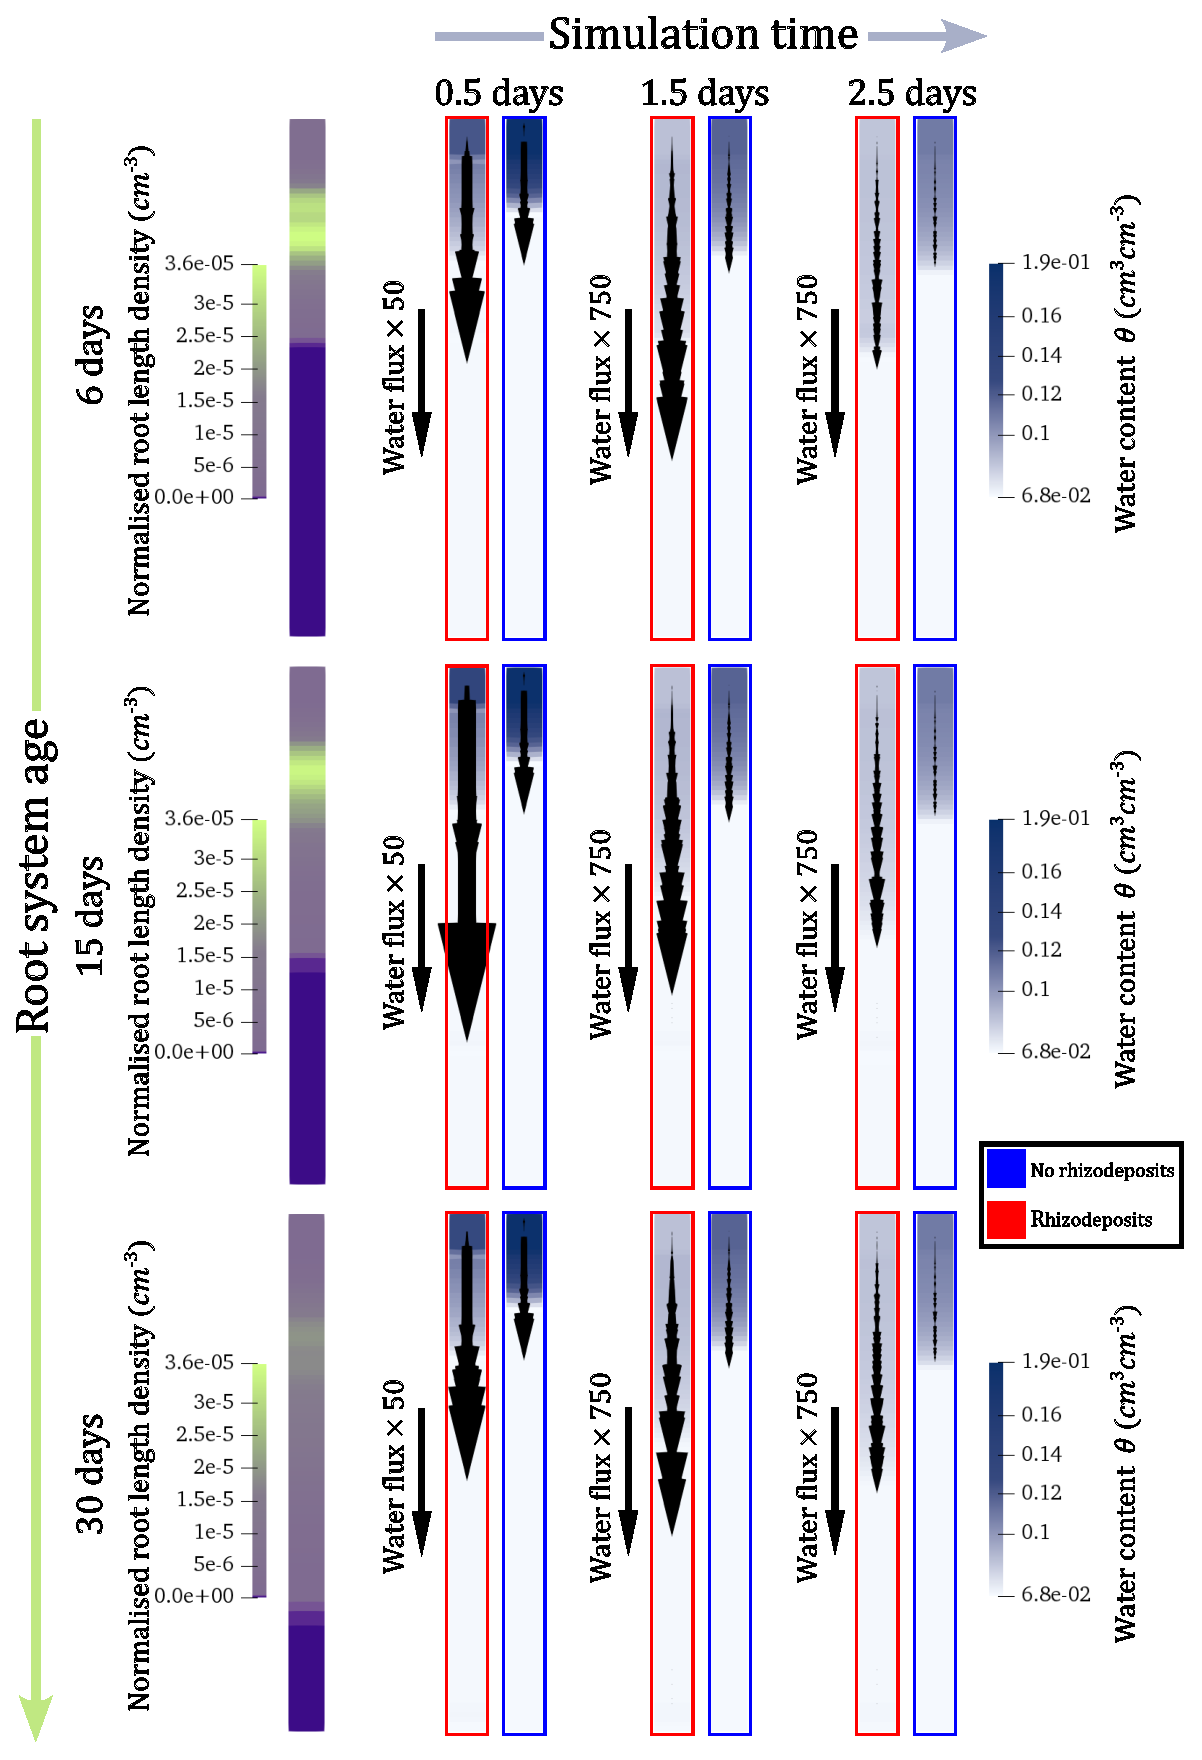
\includegraphics[width = 0.75\linewidth, keepaspectratio]{madrid_1_event.eps}
	\caption{The influence of rhizodeposits on the evolution of soil water content and flux over time under the 3-event pattern of the low-rainfall regime. The figures of the leftmost column shows the normalised root length density profiles of each plant with age increasing downwards. The remaining columns show snapshots of the water content dynamics (with and without rhizodeposits) at different time points of the simulation, where each row relates to soil vegetated by the roots of a different age of plant. The arrows illustrate the strength of the flow at each time point of the various conditions}
	\label{figure: madrid_1_event_fluxes}
\end{figure}

\begin{figure}
	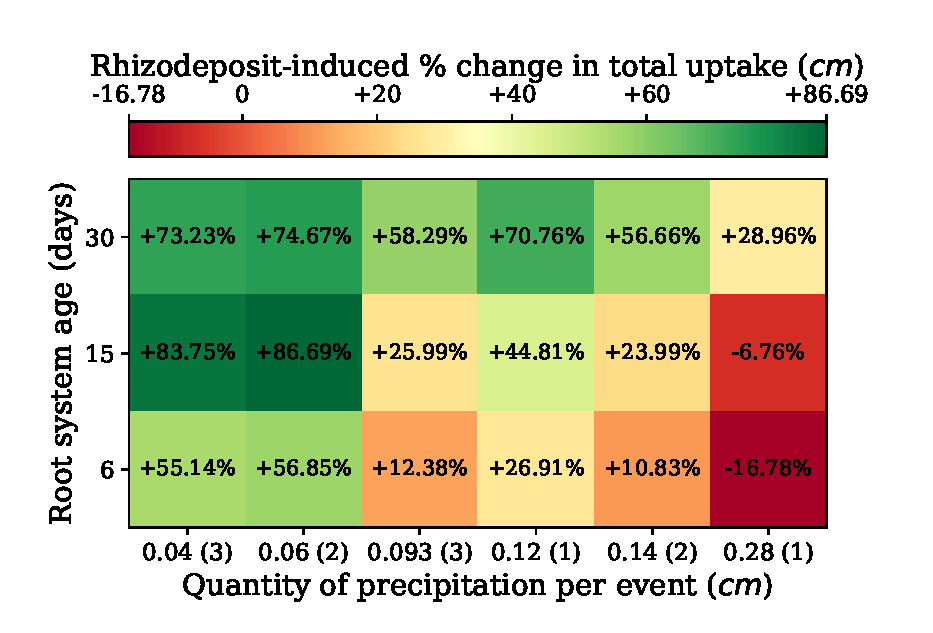
\includegraphics[width = 1.0\linewidth, keepaspectratio]{age_vs_rain_per_event.eps}
	\caption{The strength of the positive or negative effect of rhizodeposits on total water uptake of a root system in relation to root system age/depth and the quantity of precipitation delivered in each rainfall event of the precipitation regime.}
	\label{figure: uptake_age_intensity}
\end{figure}

\section{Discussion}

\subsection{Understanding the mixed impact of rhizodeposit-facilitated infiltration on root water uptake}
Mucilage from wheat has been shown to have a surfactant affect when present in the soil water solution~\citep{read2003plant}, and the effect of this within the water transport model~\eqref{model: water transport} is to increase the soil hydraulic conductivity and alter the water retention curve so that the downward flux of soil water is facilitated. As a result, in our simulations where rhizodeposits were present, water infiltrated more quickly after the onset of precipitation, and this explains the reductions in evaporation rate that were observed. Moreover, for an interval of time during and after rainfall, the rhizodeposit-induced early arrival of water to the root zone promoted the higher uptake rate compared to soils without rhizodeposits. For less intense rainfall events, the gradients in water potential that develop between the more saturated surface and the drier rooted zone are less severe and the total amount of water delivered is smaller. Consequently, in these simulations the rhizodeposit-facilitated infiltration remained gradual enough, and the quantities of water that arrived early to the uptake zone sufficiently small, so that the shallower-rooted 6-day and 15-day old plants could enjoy rhizodeposit-boosted uptake rates for the entire simulation time, and not overly suffer from water bypassing their roots.

As the rates of rainfall during each event of our simulations were increased, however, the gradients driving  water flux became greater and with time the added influence of rhizodeposits caused larger quantities of water to more quickly reach greater depths, thus becoming inaccessible to the root systems of the 6 and 15-day old plants. As a result, despite an early boost, uptake rates sooner or later dropped below those observed when rhizodeposits were not present~(Figure~\ref{figure: Madrid_precip_evap_up}), and their net effect on total water uptake can became negative~(Figure~\ref{figure: uptake_age_intensity}). 

The deeper root system possessed by the 30-day old plant meant that when rhizodeposits facilitated the transport of water to greater depths, it still remained accessible to the plant. Because of this, there was no trade off between reduced evaporation losses and a loss of water in the downward direction, and uptake rates with rhizodeposits are consistently higher than if there were no rhizodeposits present. It should be noted though that if, as reported for some species, root axial hydraulic conductivity decreases with root depth~\cite{clement2022root}, then this more unconditional benefit of rhizodeposits to deeper root systems may no longer hold. 

In summary, the findings of this study suggest that the consequences on plant water uptake of infiltration-facilitating rhizodeposits may not be universally positive and depend upon the precipitation or irrigation conditions considered. Specifically, if total precipitation over a given time arrives in fewer more intense events, then the uptake of less developed or naturally shallow root systems may be hindered by excessive surfactant-induced acceleration of downward water transport. This is consistent with knowledge on optimal irrigation practices for soils that exhibit generally high infiltration rates, where methods that promote more gradual surface water application are promoted in order to avoid losses by leaching~\citep{blackwell2000management, alhammadi2013irrigation}. Nevertheless, in environments where precipitation is less intense and more regular, rhizodeposits that facilitate infiltration are more likely to improve water availability and have a positive influence on uptake and crop performance~\citep{oostindie2010influence, chaichi2015surfactant}.            
  
\subsection{Macroscopic uptake modelling for root systems of differing biomass}
In this work, a so-called macroscopic approach~\citep{vsimuunek2009modeling, cai2018parameterization} was taken to incorporate root water uptake into the model for rhizodeposit-influenced soil water transport~\eqref{model: water transport}. The uptake function~$S$ integrates over the soil domain to give the transpiration rate of the plant, with adjustments made for local soil water stress. The potential contribution to this transpiration rate from each region of the soil domain is weighted according to the normalised root length density function~$NRLD$, and~$NRLD$ is formulated so that for any root system it integrates to 1 over the entire soil domain. For smaller root systems, the vegetated region of the domain, where the~$NRLD$ function takes non-zero values, will be smaller. Hence, in order to have a unit integral over the soil, these~$NRLD$ functions of smaller root systems have to reach larger values than those corresponding to bigger root systems who take non-zero values over a greater portion of the domain. If the transpiration rate is the same for the plants of both the smaller and larger root systems, then this means that if water spends more time in the shallower depths, which contain the roots of both the smaller and larger root systems, then under the macroscopic uptake function the uptake rate of the smaller root system will be greater than that of the larger. In our model, the transpiration rate associated to each root system increases with age in accordance with the data on basal crop coefficients in~\citep{allen1998crop}. However, this increase is not enough to counteract this effect of the normalised root length density and, under the conditions of more intense rainfall and without rhizodeposits to boost the downward flow of water, uptake rates and total uptake are greater for the 15-day old root system than the 30-day old one. This feature of the macroscopic approach means that model~\eqref{model: water transport} may underestimate the uptake of larger root systems. One method of rectifying this is would be to simultaneously model water flow within the root and shoot system as well as the soil, with a boundary condition between the two domains for the passage of water into the root cells. However, this method is very computationally expensive at large scales. If continuing with macroscopic $NRLD$-based uptake terms going forward, then the transpiration rates in~$S$ needs to be formulated so that they increase with increases in the biomass of roots and corresponding shoots and leaves above-ground.   

\subsection{Rhizodeposits for resilient crop ideotypes}
The Green Revolution of the 1960s, with the increased use of chemical fertilisers, pesticides and precise irrigation, shifted the attention of crop breeders towards the question of maximising yield under conditions where stresses from water and nutrient shortages or competition were minimal~\citep{preece2020return}. This approach led to a focus on optimal above ground traits, where one direction was to breed for crops that maximised the ratio of harvestable above ground biomass to total above ground biomass (the harvest index)~\citep{richards1993improving}. Since progress in this aspect rapidly became marginal, improvements to total above ground biomass were then sought and achieved through breeding for rapid leaf area development, to reduce evaporation losses from the soil, and enhanced leaf-level water use efficiency. Within the context of roots, however, the aim of many was to maintain root development at the necessary minimum so as to maximise resource allocation to harvestable biomass under ideal growing conditions~\citep{condon2004breeding}. Nevertheless, with the increasing incidence of global drought, breeding strategies for resilient crops have come to also consider more developed root system architectures for boosting water use efficiency. Genes have been identified that control gravitropic response and radial growth~\citep{hafeez2024breeding} and there is a consensus that increasing rooting depth should be the target of breeders. This is firstly because it allows rain-fed crops to access deep stores of water during periods of drought~\citep{lynch2013steep, uga2013control}, and secondly because, in wheat systems specifically, root arrival at theses deep water stores tends to coincide with grain-filling season thus boosting biomass before harvesting~\citep{palta2011large, wasson2012traits, ober2021wheat}.

%The results of this work suggest that root rhizodeposits, with a chemical composition that makes them act as surfactants, can reduce evaporation losses from the soil and improve uptake performance of deeply rooted systems. 

Moreover, as mentioned in a previous section, other rhizodeposits have been shown to improve retention of water (CITATION NEEDED) and facilitate rhizosphere colonisation by potentially symbiotic mycorrhizal fungi and bacteria~\cite{iannucci2021relationships}. Evidence has been shown of a genome effect on rhizodeposit and microbiome features~\citep{iannucci2021relationships}, and it has been tentatively proposed that crops could be bred to promote the development of microbiomes that are specifically beneficial under certain stresses~\cite{ober2021wheat}. Despite this, however, few breeding programmes are yet to incorporate exudate characteristics in there selections~\citep{preece2020return}. This is because the interactions between root rhizodeposits and other actors in the microbiome are very complex and vary in nature between plant growth stages~\citep{bakker2012harnessing,oburger2018sampling}. Moreover, non-destructively extracting rhizodeposits from roots grown in the field is massively challenging, and there are also issues with the more simple approach of extracting rhizodeposits from roots grown in hydroponic systems, as it is doubtful if their observed properties would be the same if extracted from roots grown in soil~\citep{oburger2018sampling}. Both of these factors mean that high throughput methods of effectively verifying that a given crop genotype induces the microbiome characteristics they are purported to require development. The same is true when it comes to models for validating the effects of these rhizodeposit and microbiome features on processes like water and nutrient availability. Within the modelling field there are differing approaches to incorporating rhizodeposit influence into models for water transport and uptake. Like in~\citep{vogel1996hydrus, karagunduz2001influence}, our model assumes that the effect of rhizodeposit induced changes on contact-angle and surface tension can be incorporated into water retention~\eqref{model: water retention} and hydraulic conductivity~\eqref{model: hydraulic conductivity} by using the same effective saturation function~\eqref{model: effective saturation} with an appropriately scaled air entry pressure term~\eqref{model: alpha vs rhizodeposits}. However, this was not the case in~\citep{cooper2017fluid, cooper2018effect}, where the influence of root exudates was incorporated into Richards equation through a rigorous multi-scale derivation and the effect of increasing contact angle resulted in retention and conductivity curves that no longer resembled the common functions of~\cite{brooks1964hydrau} or~\cite{mualem1976new} and~\cite{van1980closed}. Additionally, in~\citep{landl2021modeling} the effect of mucilage on water uptake is modelled, and a third different method, that of~\cite{kroener2014nonequilibrium}, is used to incorporate mucilage-induced changes in water retention. In both our work and that of~\cite{landl2021modeling} many model parameters had to be taken from a wide range of existing publication and this also indicate the challenges in model calibration that arise from the fact that extracting exudates and reliably observing their effects is a complicated and expensive process. 

The results of this work suggest that root rhizodeposits, with a chemical composition that makes them act as surfactants, can reduce evaporation losses from the soil and improve uptake performance of deeply rooted systems. However, for the reasons above, the insights that can be drawn from this are modest and much work is required before such insights can be incorporated into the more simple large scale models for crop yield.
For breeding for rhizodeposit characteristics to be a viable option, the future work is needed to progress to a stage where: there is more consensus on the correct approach to model the effect of rhizodeposit induced changes to soil hydraulics on water transport, experiments for the effect of exudates on the hydraulic parameters of these models can be more easily carried out and, finally, genotypes can be identified which correspond to these exudate effects. 

 

%\begin{figure}
%	\centering
%	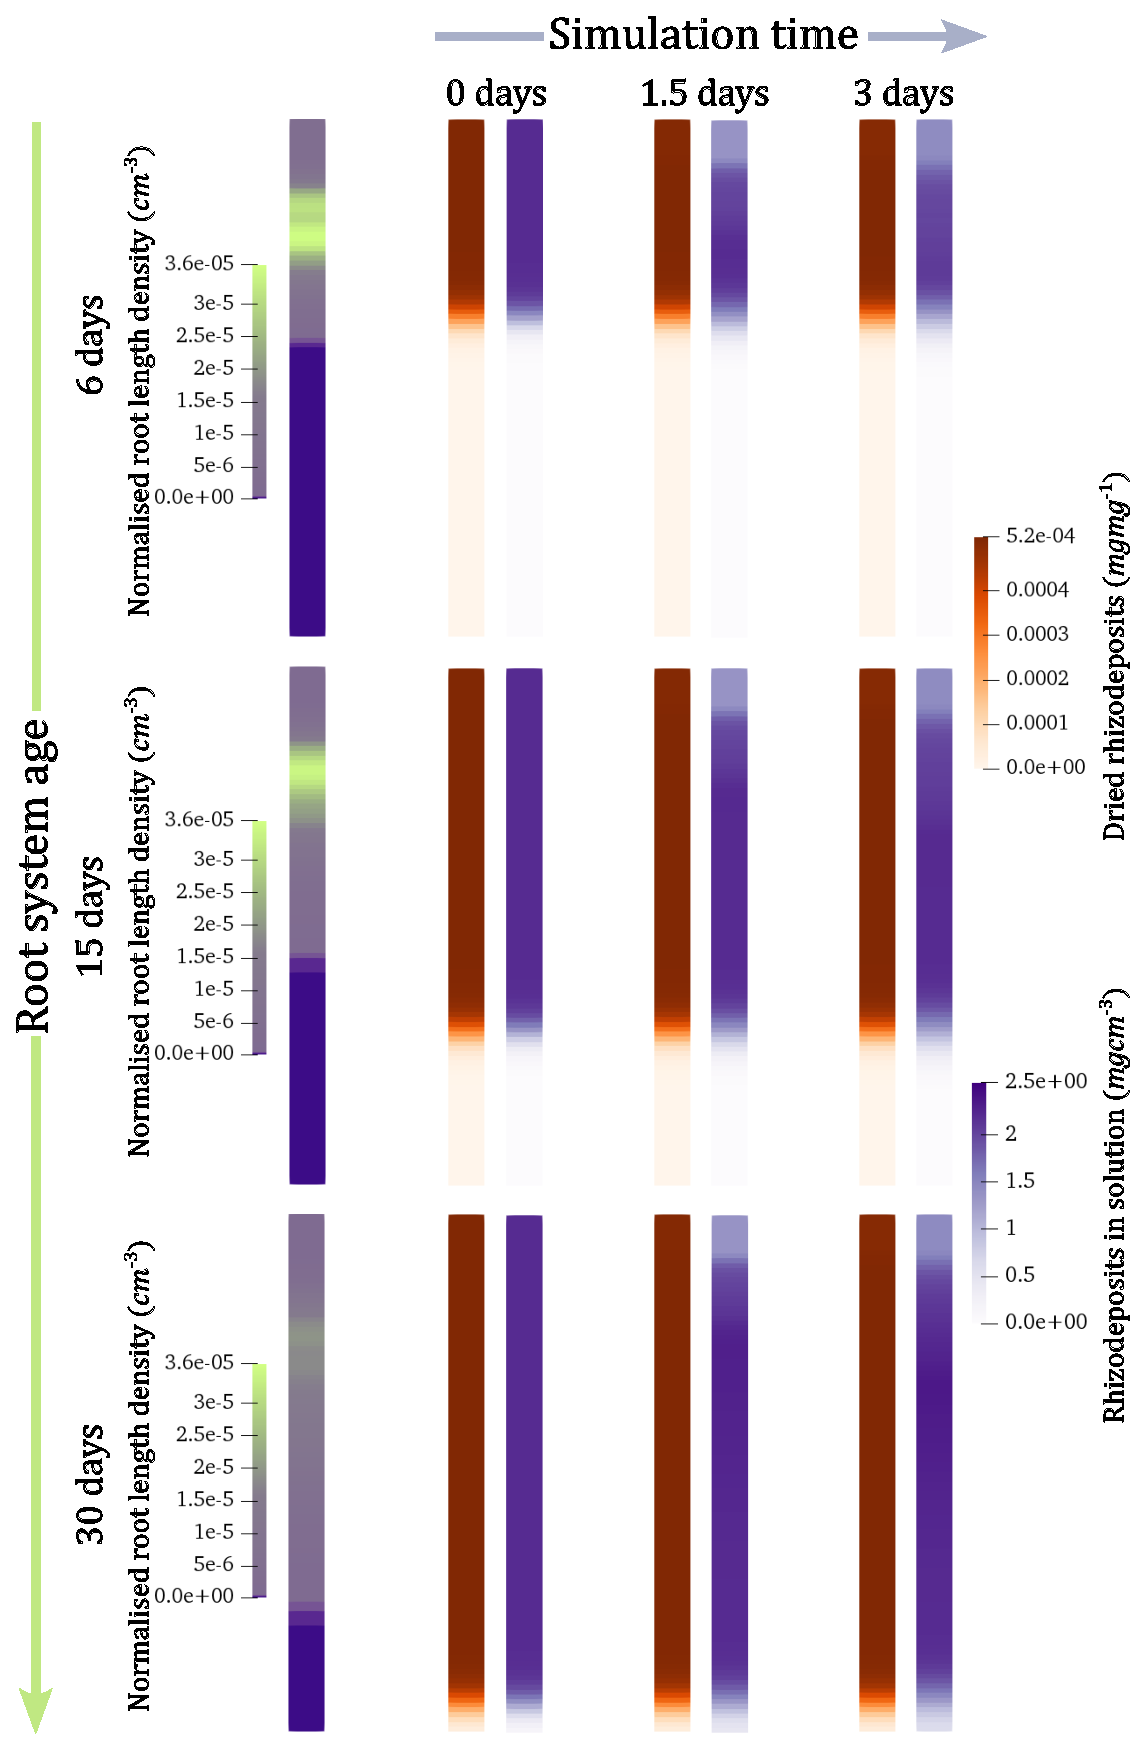
\includegraphics[width = 0.75\linewidth, keepaspectratio]{rhizodeposit_profiles_almeria_3_events.eps}
%	\caption{Almeria rhizodeposits}
%	\label{figure: almeria_3_events_rhizodeposits}
%\end{figure}
%
%\begin{figure}
%	\centering
%	\includegraphics[width = 0.75\linewidth, keepaspectratio]{rhizodeposit_profiles_madrid_1_event.eps}
%	\caption{Madrid rhizodeposits}
%	\label{figure: madrid_1_event_rhizodeposits}
%\end{figure}

\bibliographystyle{chicago}
\bibliography{rhizodeposit_influence_bibliography}

\end{document}	